\documentclass[twoside,11pt]{scrbook}

% Establece el español como idioma del documento.
\usepackage[spanish,es-tabla]{babel}
\usepackage[utf8]{inputenc}

% Activa los enlaces dentro del documento (recuadros rojos en el PDF).
\usepackage{hyperref}

% Mejora el formato de las citas.
\usepackage{cite}

% Permite definir términos y acrónimos.
\usepackage[acronym]{glossaries}
\makeglossaries
 
% Ajusta los márgenes establecidos en la guía de estilos para TFM de la EPS.
\usepackage[
  inner=3cm,
  outer=2.5cm,
  top=2.5cm,
  bottom=2.5cm
]{geometry}

% Permite definir colores como variables
\usepackage{color}

% Definición de colores para el documento.
%    Nota: El rango de los colores va de 0 a 1.

\definecolor{dgreen}{rgb}{0,0.6,0}
\definecolor{mauve}{rgb}{0.58,0,0.82}


% Permite insertar pdf.
\usepackage{pdfpages}

% Permite añadir bloques de código.
\usepackage{listings}


% Sintaxis de Golang, se ha de importar después de listings.

\usepackage{./conf/languages/golang}

\lstset{
  frame=tb,
  aboveskip=3mm,
  belowskip=3mm,
  showstringspaces=false,
  columns=flexible,
  basicstyle={\small\ttfamily},
  numbers=none,
  numberstyle=\tiny\color{gray},
  keywordstyle=\color{blue},
  commentstyle=\color{dgreen},
  stringstyle=\color{mauve},
  breaklines=true,
  breakatwhitespace=true,
  tabsize=4
}


% Información acerca del trabajo
\title{Mi Trabajo Final de Máster} 
\author{David Peinado} 
\date{Marzo 2018}
\publishers{Universidad de Alicante}

% Añade las definiciones de acrónimos.
\newglossaryentry{gutc}{
	name=gUTC,
	description={GLOSSARY Coordinated Universal Time}}
	
\newglossaryentry{gadt}{
	name=gADT,
	description={GLOSSARY  Atlantic Daylight Time}}
	
\newglossaryentry{gest}{
	name=gEST,
	description={GLOSSARY Eastern Standard Time}}
 
\newglossaryentry{autc}{
	type=\acronymtype,
	name={aUTC},
	description={ACRONYM Coordinated Universal Time},
	first={ACRONYM Coordinated Universal Time (aUTC)\glsadd{autc}}} 
	% see=[Glossary:]{autc}} % añadir si tiene referencia en glosario

\newglossaryentry{aadt}{
	type=\acronymtype, 
	name={aADT}, 
	description={ACRONYM Atlantic Daylight Time}, 
	first={ACRONYM Atlantic Daylight Time (aADT)\glsadd{aadt}}}

\newglossaryentry{aest}{
	type=\acronymtype, 
	name={aEST}, 
	description={ACRONYM Eastern Standard Time}, 
	first={ACRONYM Eastern Standard Time (aEST)\glsadd{aest}}}


% ----------------------------- DOCUMENT BEGINS -----------------------------
\begin{document}

% -------------- COVER --------------
\begin{titlepage}

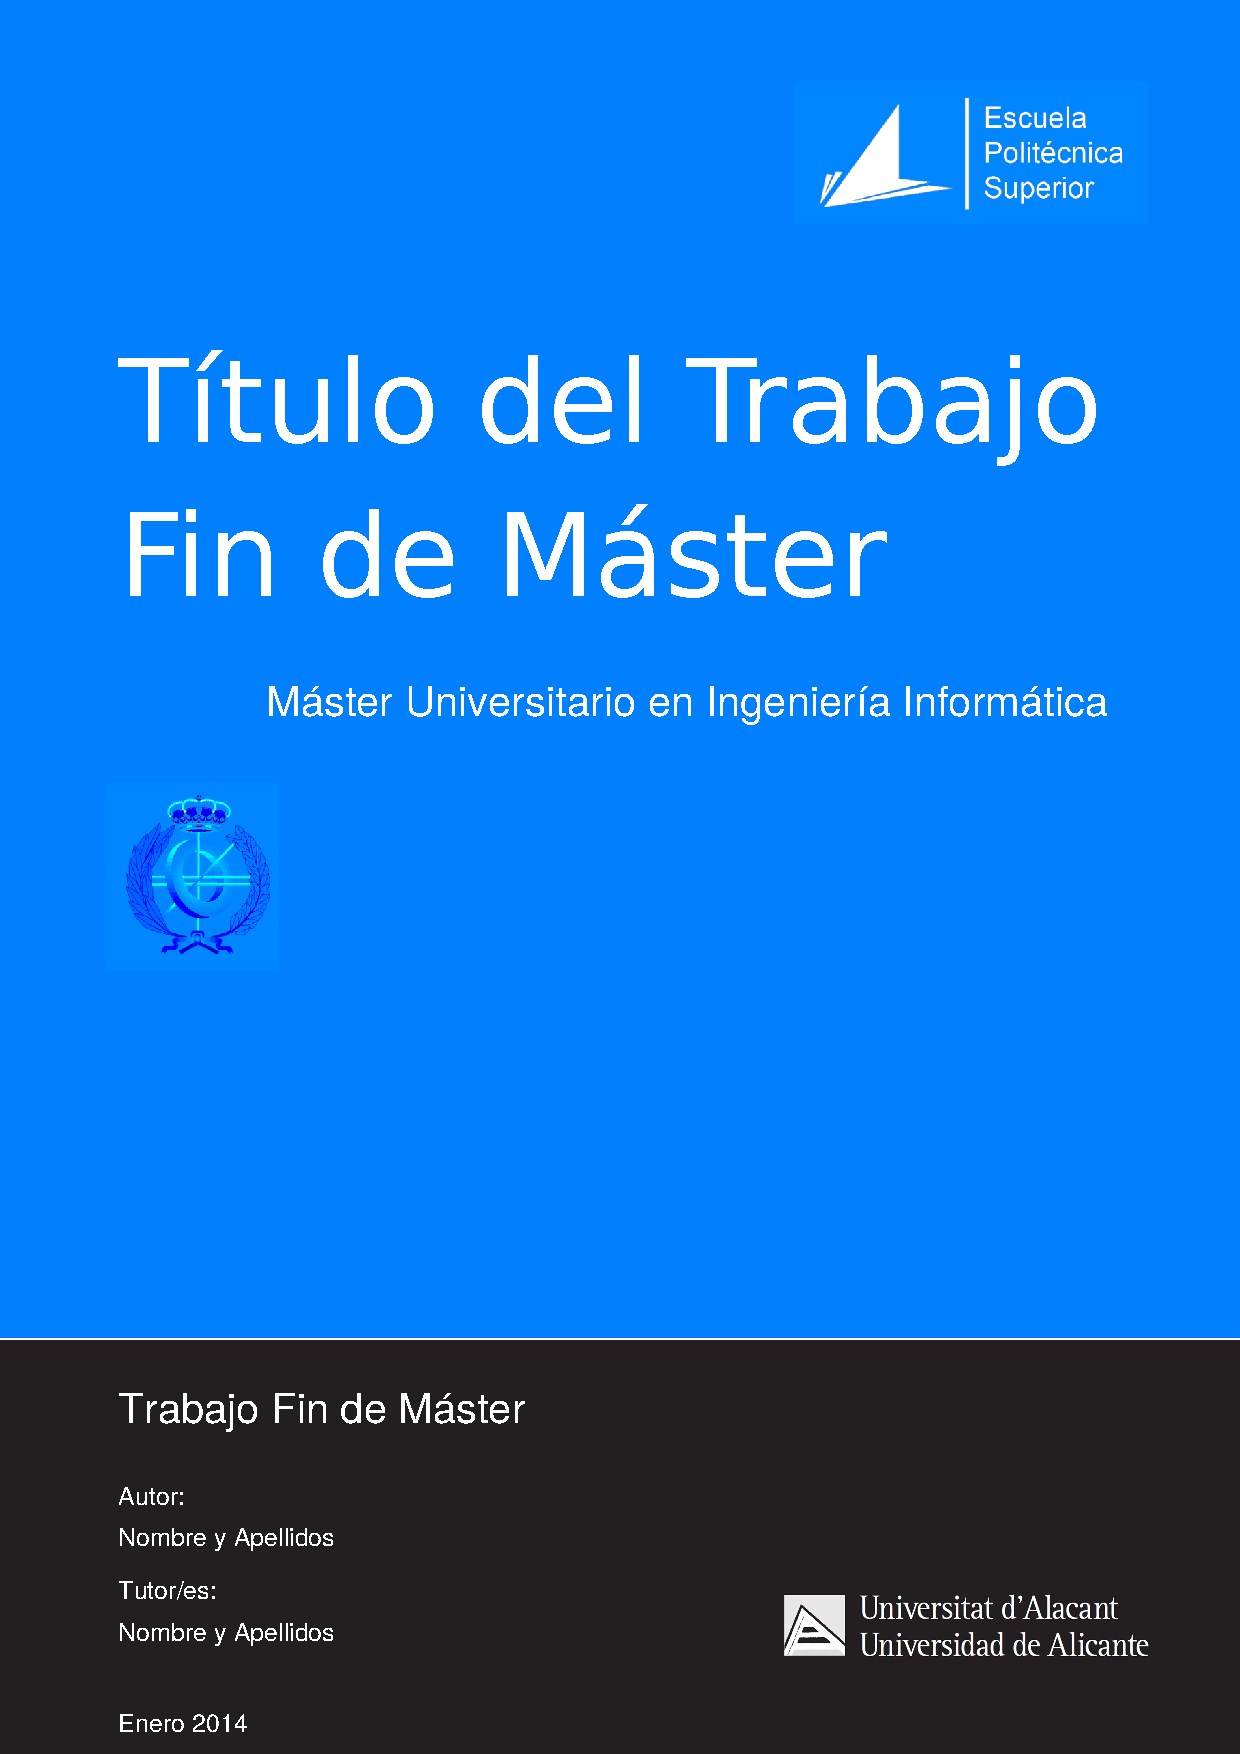
\includepdf[pages={1},fitpaper=true]{cover/cover.pdf}

\end{titlepage}
\pagecolor{white}


% -------------- TITLE --------------
\maketitle


% -------------- FRONT MATTER --------------
\frontmatter

\chapter*{Preámbulo}

Justificación y Objetivos: se describirán la motivación que ha originado la
realización del TFG/TFM, así como de una breve descripción de los objetivos
generales que se quieren alcanzar con el trabajo presentado.


\chapter*{Resumen} 

A brief summary of the project goes here.  


\chapter*{Agradecimientos} 

Agradecimientos: se podrá añadir las hojas necesarias para realizar los
agradecimientos, a veces obligatorios, a las entidades y organismos colaboradores.

\tableofcontents 
\listoffigures 
\listoftables
\printglossary[title={Lista de acrónimos}, type=\acronymtype]
\printglossary[type=main]

\chapter*{}
\setlength{\leftmargin}{0.5\textwidth}
\setlength{\parsep}{0cm}
\addtolength{\topsep}{0.5cm}
\begin{flushright}
\small\em{
Se podrá añadir una única hoja con dedicatorias,\\
su alineación será derecha y centradas\\
de forma distribuida en la página
}
\end{flushright}


\chapter*{}
\setlength{\leftmargin}{0.5\textwidth}
\setlength{\parsep}{0cm}
\addtolength{\topsep}{0.5cm}
\begin{flushright}
\small\em{
Se podrá añadir una única hoja con citas,\\
su alineación será derecha y centradas\\
de forma distribuida en la página
}
\end{flushright}



% -------------- MAIN MATTER--------------
\mainmatter
\glsresetall % resetea glosario y acrónimos por si se han utilizado antes.

\chapter{Introducción} 
\label{ch:intro}

Introducción: donde se hará énfasis a la importancia de la temática, su vigencia y actualidad; se planteará el problema a investigar, así como el propósito o finalidad de la investigación

Usando el acrónimo \gls{autc}.\\
Ahora usamos \gls{aadt}.\\
Y por último \gls{aest}.

\lstinputlisting[
    language=golang,
    inputencoding=latin1,
    caption={[Makefile]Makefile, foobar},
]{./code/golang_example.go}


\section{Estado del arte}

Marco teórico o Estado del arte: se hará mención a los elementos conceptuales
que sirven de base para la investigación, estudios previos relacionados con el
problema planteado, etc.

\chapter{Objetivos} 
\label{ch:obj} 

Objetivos: se establecerá el objetivo general y los específicos.

Usando el término \gls{gutc}.\\
Ahora usamos \gls{gadt}.\\
Y por último \gls{gest}.

\section{Objetivos específicos}
Ahora usamos el acrónimo \gls{autc} por segunda vez.

\lstinputlisting[
    language=python,
    inputencoding=latin1,
    caption={[Makefile]Makefile, foobar},
]{./code/python_example.py}


\chapter{Metodología} 
\label{ch:method}

Metodología: se indicará el tipo o tipos de investigación, las técnicas y los procedimientos que serán utilizados para llevarla a cabo; se identificará la población y el tamaño de la muestra así como las técnicas e instrumentos de recolección de datos.

\chapter{Cuerpo del documento} 
\label{ch:body}

Cuerpo del trabajo: incluirá los resultados de la investigación o trabajo, así como el análisis y la discusión de los mismos.\showthe\font


\chapter{Conclusión} 
\label{ch:method}

Conclusiones: obligatoriamente se incluirá una sección de conclusiones donde se
realizará un resumen de los objetivos conseguidos así como de los resultados
obtenidos si proceden

\section{Líneas futuras}

Líneas de investigación o proyectos abordables tras la realización del trabajo.


% -------------- BACK MATTER --------------
\backmatter
\nocite{*} % incluye las referencias que no se hayan citado.
\bibliographystyle{apalike}
\setbibpreamble{Bibliografía y referencias: se incluirá también la relación de obras y materiales consultados y empleados en la elaboración de la memoria del TFG/TFM. La bibliografía y las referencias serán indexadas en orden alfabético (sistema nombre y fecha) o se numerará correlativamente según aparezca (sistema numérico). Se empleará la familia 1 como tipo de letra. Podrá utilizarse cualquier sistema bibliográfico normalizado predominante en la rama de conocimiento, estableciéndose como prioritarios el sistema ISO 690, sistema APA (American Psychological Association) o Harvard (no necesariamente en ese orden de preferencia).\\}

{\sffamily
\bibliography{./bibliography/bibliography}
}

\appendix

\end{document} 